\documentclass{TDP003mall}



\newcommand{\version}{Version 1.0}
\author{Johan Törner, \url{daniel.o.persson@liu.se}\\
  Linus Nordin, \url{emanuel.kinberger@liu.se}\\}
\title{Installationsmanual}
\date{2023-09-21}
\rhead{Linus Nordin\\
Johan Törner}



\begin{document}
\graphicspath{ {./images/} }

\projectpage
\section{Revisionshistorik}
\begin{table}[!h]
\begin{tabularx}{\linewidth}{|l|X|l|}
\hline
Ver. & Revisionsbeskrivning & Datum \\\hline
1.0 & Första Versionen & 230921 \\\hline
\end{tabularx}
\end{table}


\section{Inledning}

Denna manual körs på ett Debian-baserat operativsystem, t.ex Ubuntu.\\
För att kunna arbeta portfolio-sidan så krävs en del dependencies.\\
Först behövs någon form av text-hanterare.\\

Alla kommandon körs genom Linux-terminalen, som öppnas med Ctrl-Alt-T.\\



\section{Python3}
Det första som måste installeras är Python3.\\
Python-versionen som används inom detta projekt är 3.10\\ 
Kommandot för att installera Python3;\\\\
\textbf{sudo apt-get install python3}\\\\
Man bör kolla att python3 och pip är installerat med\\\\
\textbf{python3 -m pip --version}\\\\
Ibland så kan det bli så att pip inte installeras.\\
Om terminalen ger en error så kan pip installeras med följande kommando\\\\
\textbf{sudo apt-get install pip}\\\\
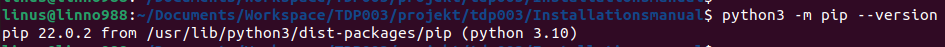
\includegraphics[scale=0.5]{pip_version}

\section{Git}
Versionshanterar-systemet Git är också ett krav.\\ 
Vi kan installera Git genom terminalen med kommandot;\\\\
\textbf{sudo apt-get install git-all}\\\\
Då borde Git vara installerat, man kan kolla att det gick rätt med versionskommandot;\\\\
\textbf{git version}\\\\
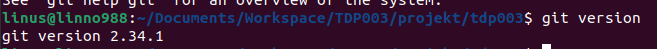
\includegraphics[scale=0.5]{git_version}

\section{Emacs}
Installationen av Emacs sker genom terminalen.\\
I ett Debian-baserat system (Ubuntu, till exempel) så används\\\\
\textbf{sudo apt-get install emacs}\\\\
Bekräfta sedan att emacs är installerat med\\\\
\textbf{emacs -version}\\\\
Sedan kan man köra emacs genom terminalen eller så kan man öppna en GUI för emacs.\\\\
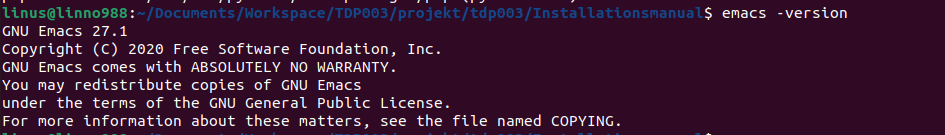
\includegraphics[scale=0.5]{emacs_version}


\section{Visual Studio Code}
Visual Studio Code installeras med kommandot\\\\
\textbf{sudo apt-get install code}\\\\ 
Sedan kör man VSC med\\\\
\textbf{code}
\subsection{Python för VSC}
När VSC är installerad och öppnad så bör man installera Python extensionen\\
På vänstra delen av VSC så finns det en rad med knappar, tryck på den för Extensions.\\
Sök sedan efter "Python" och installera den som helt enkelt heter "Python" och kommer från Microsoft\\
Då installeras även Pylance.\\\\
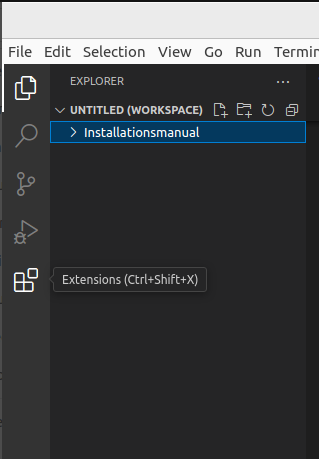
\includegraphics[scale=0.5]{extensions}


\section{Flask}\\
För att kunna arbeta med Python inom webbsidan så måste vi ha Flask.\\
Jinja2 behövs för att kunna rendera sidan, men vi kommer få med Jinja2 med installation av Flask.\\ 
Vi använder oss av Pip för att installera Flask.\\\\
\textbf{pip install Flask}\\\\
Nu är både Flask och Jinja2 installerat.\\
\subsection{Att köra Flask}
För att köra Flask så bör man stå i katalogen för projektets app.py och sedan köra kommandot\\\\
\textbf{flask run}\\\\
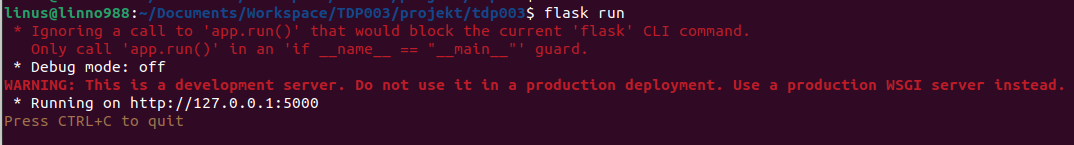
\includegraphics[scale=0.4]{flask_run}


\end{document}
